\documentclass[12pt,a4paper]{article}
\usepackage[utf8]{inputenc}
\usepackage[T1]{fontenc}
\usepackage[francais]{babel}
\usepackage{amsmath}
\usepackage{amsfonts}
\usepackage{amssymb}
\usepackage{graphicx}
\usepackage[top=2.00cm]{geometry}
\usepackage{titlesec}
%%modif des titres de section diminuer la taille
\graphicspath{{C:/Users/Sylvain/AppData/Roaming/texstudio/templates/user/}}
\renewcommand{\thesection}{\Roman{section}}
\titleformat{\section}
{\normalfont\bfseries\Large\scshape}{\thesection}{1em}{}
\titleformat{\subsection}
{\normalfont\bfseries\large}{\thesubsection}{1em}{}

\makeatletter
\def\@maketitle{
	
	\begin{center}
		% NoLogo
		% \vspace*{+2cm}
		
		% Corner Logo
		% \begin{flushright}
		%  
\includegraphics[width=40mm]{logo_corner}\\[4ex]
		% \end{flushright}
		
		% Top Logo
		
\includegraphics[scale=0.3]{logo_top}
		
		
		{\LARGE \@title }\\[4ex]
		{\large \@author}\\[4ex]
		{\large \@date}\\[8ex]
		\rule{\linewidth}{0.4pt}
	\end{center}
}
\makeatletter

\author{CHARNAY Valentin, FINOT Sylvain}
\title{Compte rendu de TP :\\[4pt] \scshape Oscillateurs }
\date{\today}
\begin{document}
	\maketitle
	\section{Modélisation d'un frottement solide}
	L'équation d'un circuit RLC est donnée par :
	$$L\dfrac{d^2q}{dt^2}+R\dfrac{dq}{dt}+\dfrac{q}{C}=0$$
	Si on ajoute des diodes dans le circuit, cela revient à les considérer comme des interrupteurs qui sont ouverts à partir d'une certaine tension de seuil et fermés si la tension est inférieure à cette tension de seuil.\\
	On peut alors écrire
	$$L\dfrac{d^2q}{dt^2}+R\dfrac{dq}{dt}+\dfrac{q}{C}=U_s$$
	Là où en mécanique on aurait une équation de la forme :
	$$m\ddot{x}+(\rho\dot{x})+kx=f_c$$
	%Lorsque la tension aux bornes des diodes est inférieure à la tension de seuil, le courant ne passe pas $\implies$ on coupe les petites oscillations.
	
	Le frottement n'est pas réellement/purement solide à cause de la présence de la résistance qui joue le rôle de coefficient de frottement visqueux (par analogie à un système mécanique).
	$$\left( R\dfrac{dq}{dt}\iff\rho\dot{x}\right) = 0 \quad \text{Si purement solide}$$
	On peut étudier rapidement cette équation différentielle.
	\begin{equation*}
	\ddot{q}+\dfrac{R}{L}\dot{q}+\dfrac{1}{LC}q=\dfrac{U_s}{L}
	\end{equation*}
	On cherche une solution particulière, il y en a une évidente : 
	$$q=U_sC$$
	On cherche maintenant une solution générale, pour cela on calcule le déterminant du polynôme caractéristique :
	$$\Delta=\left(\dfrac{R}{L}\right)^2-\dfrac{4}{LC}$$ 
	On pourrait traiter tous les cas, mais on s'intéresse ici aux solutions pseudo-périodiques (i.e $\Delta<0$)\\[4pt]
	On pose alors : $r_{\pm}=\dfrac{1}{2}(-\dfrac{R}{L}\pm i\sqrt{-\Delta})$\\
	La solution de cette équation différentielle est de la forme :
	\begin{align*}
	q &= q_G + q_P\\
	&=A \exp(r_+t)+B\exp(r_-t)+U_sC\\
	&=\exp\left(-\dfrac{R}{2L}t\right)\left[A\exp(\dfrac{i\sqrt{-\Delta}}{2}t)+B\exp(\dfrac{-i\sqrt{-\Delta}}{2}t)\right]+U_sC
	\end{align*}
	Équation que l'on peut aussi écrire sous la forme :
	\begin{equation}
	q=\exp\left(-\dfrac{R}{2L}t\right) \times A' \cos(\dfrac{\sqrt{-\Delta}}{2}t+\phi)+U_sC
	\end{equation}
	Ou $A'$ et $\phi$ sont des constantes que l'on peut déterminer à partir de conditions (conditions initiales par exemple).\\
	On peut alors trouver l'équation sur le courant : $I(t)=\dot{q}(t)$
	\section{Oscillateurs couplés}
	\subsection{Étude théorique}
	Les solutions peu amorties ont une dépendance temporelle en (Cf énoncé)
	$$\cos\left(\dfrac{\omega'+\omega''}{2}t\right)\cos\left(\dfrac{\omega'-\omega''}{2}t\right)$$
	avec
	$$\omega'=\sqrt{\dfrac{1}{LC}} \qquad \omega''=\sqrt{\dfrac{1}{LC}+\dfrac{2}{LC'}}$$
	N'ayant pas de définition précise du sens de couplage fort et faible, on prendra comme hypothèse que dans la limite où le couplage tend vers 0, on peut considérer les systèmes comme indépendants. Par conséquent, cela signifie que si le couplage est faible, les pulsations ne sont autres que les pulsations des systèmes vus séparément. D'après cette hypothèse et d'après les expressions des pulsations, on en déduit que le couplage est fort si $\omega'$ est très différent de $\omega''$.
	\begin{align*}
	\dfrac{1}{LC}&\ll\dfrac{2}{LC'}\\
	\implies C'&\ll\dfrac{C}{2}\\
	\text{ou encore} \quad 1&\ll\dfrac{C}{2C'}\\
	\end{align*}
	\subsection{Étude expérimentale}
	$$\cos\left(\dfrac{\omega'+\omega''}{2}t\right)\cos\left(\dfrac{\omega'-\omega''}{2}t\right)$$
	\begin{align*}
	\implies
	\begin{cases}
	\dfrac{2\pi}{T_1}&=\dfrac{\omega'+\omega''}{2}\\[1em]
	\dfrac{2\pi}{T_2}&=\dfrac{\omega'-\omega''}{2}
	\end{cases}
	\iff
	\begin{cases}
	\dfrac{4\pi}{T_1}=\omega'+\omega''\\[1em]
	\dfrac{4\pi}{T_2}=\omega'-\omega''
	\end{cases}
	\end{align*}
	\begin{equation*}
	\iff
	\begin{cases}
	\omega'=2\pi\left(\dfrac{1}{T_1}+\dfrac{1}{T_2}\right)\\[1em]
	\omega''=2\pi\left(\dfrac{1}{T_1}-\dfrac{1}{T_2}\right)
	\end{cases}
	\end{equation*}
	Le terme d'amortissement est juste une exponentielle décroissante, sans doute de la forme $\exp(-R/2\rho\times t)$ (par analogie avec la mécanique).
	On obtient donc à l'oscilloscope la figure ci-dessous qui met en évidence le phénomène de battements.
	\begin{figure}[h]
		\centering
		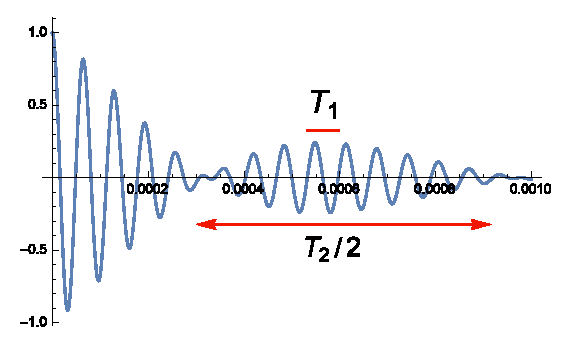
\includegraphics[width=0.7\linewidth]{couplage2.eps}
	\end{figure}
	On peut donc trouver $T_1$ et $T_2$ et ainsi calculer $\omega'$ et $\omega''$ pour les comparer aux valeurs théoriques.
	
	Par lecture à l'oscilloscope, on a :
	$T_1 = 65\mu s$ $\quad$ $T_2 = 1304\mu s$\\
	\begin{equation*}
	\implies 
	\begin{cases}
	\omega'=2\pi\left(\dfrac{1}{T_1}-\dfrac{1}{T_2}\right)\\[1em]
	\omega''=2\pi\left(\dfrac{1}{T_1}+\dfrac{1}{T_2}\right)
	\end{cases}
	\implies
	\begin{cases}
	\omega'=9,18.10^4Hz\\[1em]
	\omega''=1,01.10^5Hz
	\end{cases}
	\end{equation*}
	Les valeurs théoriques sont :
	\begin{equation*}
	\begin{cases}
	\omega'=\sqrt{\dfrac{1}{LC}}\\
	\omega''=\sqrt{\dfrac{1}{LC}+\dfrac{2}{LC'}}
	\end{cases}
	\iff
	\begin{cases}
	\omega'=\sqrt{\dfrac{1}{10,6.10^{-3}.11.10^{-9}}}\\
	\omega''=\sqrt{\dfrac{1}{10,6.10^{-3}.11.10^{-9}}+\dfrac{2}{10,6.10^{-3}.100.10^{-9}}}
	\end{cases}
	\end{equation*}
	\begin{equation*}
	\begin{cases}
	\omega'=9,26.10^4Hz\\
	\omega''=1,02.10^5Hz
	\end{cases}
	\end{equation*}
	En comparant la théorie à la pratique, on constate que les résultats sont très proches. Le petit écart s'explique par la difficulté de lecture étant donné qu'il s'agit de pseudo-période.
	
	Nous n'avons pas effectué de relevés précis dans le cas du couplage fort (que l'on obtient en augmentant la valeur de C symétriquement pour chacun des circuits RLC). On remarque tout de même que le battement disparait et laisse place à une enveloppe décroissante (l'enveloppe de l'amortissement).
\end{document}

